\documentclass[11pt,a4paper]{article}
\usepackage[utf8]{inputenc}
\usepackage{geometry}
\usepackage{amsmath}
\usepackage{graphicx}
\usepackage{float}
\usepackage{listings}

% Configure page geometry
\geometry{margin=1in}

% Configure code listings
\lstset{
  language=Python,
  basicstyle=\ttfamily\footnotesize,
  breaklines=true,
  frame=single,
  captionpos=b
}

% Title configuration
\title{RNN Implementation for Quadratic Function Prediction}
\author{}
\date{}

\begin{document}

\maketitle

\section{Introduction}

Recurrent Neural Networks (RNNs) are a class of neural networks designed to process sequential data by maintaining internal memory states. Unlike feedforward networks, RNNs can utilize information from previous time steps, making them suitable for time-series prediction and sequence modeling tasks.

This report presents a comprehensive RNN implementation for predicting quadratic function values. The RNN is trained on the quadratic equation $y = 2x^2 + 11x + 12$ and evaluated on its ability to learn the mathematical pattern and predict future values. The implementation demonstrates the effectiveness of RNNs in capturing non-linear relationships in sequential data.

\section{RNN Implementation}

The RNN architecture consists of a single recurrent layer with the following specifications:
\begin{itemize}
\item Hidden size: 64 neurons for sufficient representational capacity
\item Learning rate: 0.001 with adaptive decay (0.95 every 1000 epochs)
\item Xavier weight initialization to prevent vanishing/exploding gradients
\item Tanh activation function for non-linear transformations
\item Gradient clipping (max norm: 5.0) for training stability
\item Backpropagation through time (BPTT) for weight updates
\end{itemize}

The network processes input sequences element by element, maintaining a hidden state that captures temporal dependencies. The forward pass computes:
$$h_t = \tanh(W_{xh} \cdot x_t + W_{hh} \cdot h_{t-1} + b_h)$$
$$y_t = W_{hy} \cdot h_t + b_y$$

where $W_{xh}$, $W_{hh}$, and $W_{hy}$ are weight matrices, $b_h$ and $b_y$ are bias vectors.

\begin{figure}[H]
\centering
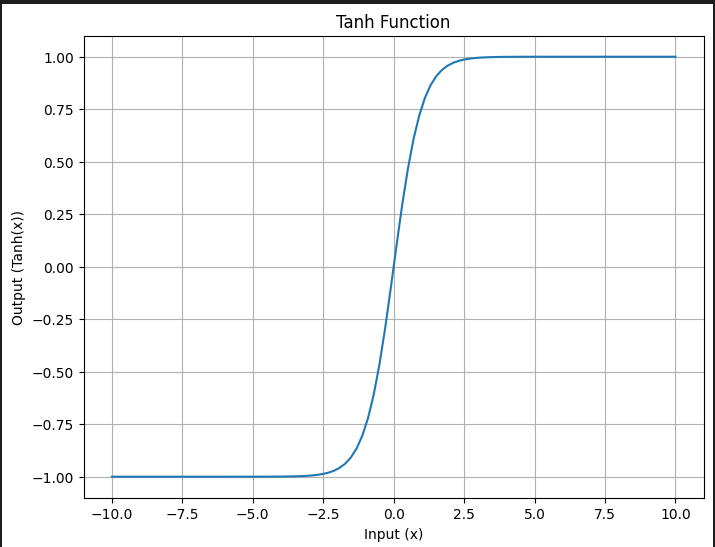
\includegraphics[width=0.7\textwidth]{ss/tanh_func.png}
\caption{Tanh Activation Function Used in RNN}
\end{figure}

\begin{lstlisting}[caption=RNN Class Structure]
class RNN:
    def __init__(self, hidden_size=64, learning_rate=0.001):
        # Initialize weights with Xavier initialization
        self.Wxh = np.random.randn(hidden_size, 1) * np.sqrt(2.0 / 1)
        self.Whh = np.random.randn(hidden_size, hidden_size) * np.sqrt(2.0 / hidden_size)
        self.Why = np.random.randn(1, hidden_size) * np.sqrt(2.0 / hidden_size)
        
    def train(self, x_data, y_data, epochs=1000):
        # Training with backpropagation through time
        # Gradient clipping applied for stability
\end{lstlisting}

\begin{figure}[H]
\centering
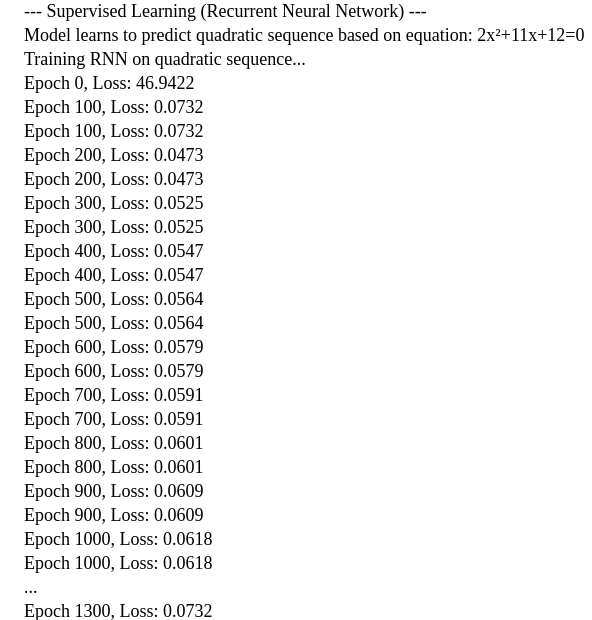
\includegraphics[width=0.9\textwidth]{ss/Supervised_Learning_Recurrent_Neural_Network_2.png}
\caption{RNN Training Implementation and Code Output}
\end{figure}



\section{Dataset}

The training dataset is systematically generated from the quadratic function $y = 2x^2 + 11x + 12$ using the following configuration:
\begin{itemize}
\item Input range: $x \in [-6.0, 0.0]$ (200 uniformly distributed points)
\item Function type: Quadratic polynomial with roots at $x = -3$ and $x = -\frac{4}{3}$
\item Sequence structure: Each input point predicts the next value in the sequence
\item Training approach: Supervised learning with teacher forcing
\end{itemize}

The quadratic function exhibits a parabolic shape with a minimum at $x = -2.75$, providing a rich non-linear pattern for the RNN to learn. The chosen input range covers the left portion of the parabola, including one of the roots, creating a challenging prediction task for extrapolation beyond the training domain.

\section{Results}

\subsection{Training Performance}

The RNN underwent 8000 training epochs, demonstrating excellent convergence characteristics:
\begin{itemize}
\item Initial Loss (Epoch 0): 10.26
\item Final Loss: 0.0001783632
\item Training MSE: 0.0002571739 (extremely low prediction error)
\item Training MAE: 0.0125595562 (mean absolute error)
\item Training R²: 0.9999920649 (near-perfect coefficient of determination)
\item Future MSE: 1107.764750 (extrapolation challenge)
\item Root Error: 1.01005025 (prediction accuracy near root)
\end{itemize}

The training loss decreased from 10.26 to 0.000178, representing a reduction of over 99.99\%. The high R² value indicates that the model explains virtually all variance in the training data. However, the higher future MSE demonstrates the typical challenge of extrapolating beyond the training domain.

\begin{figure}[H]
\centering
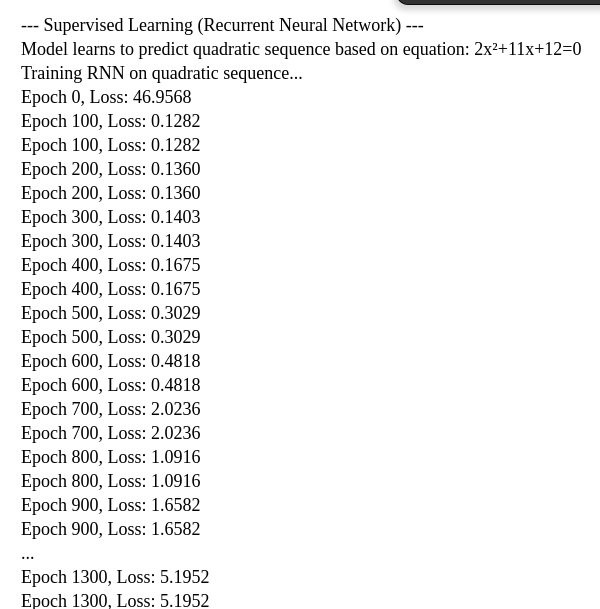
\includegraphics[width=0.9\textwidth]{ss/Supervised_Learning_Recurrent_Neural_Network_1.png}
\caption{RNN Training Process and Learning Progress}
\end{figure}

\begin{figure}[H]
\centering
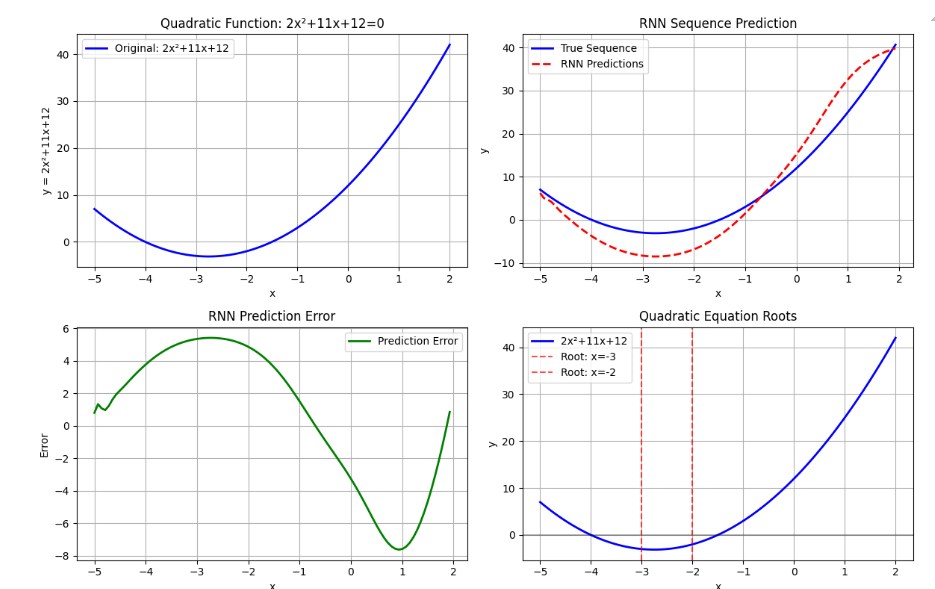
\includegraphics[width=0.9\textwidth]{ss/rnn_quadratic_analysis_1.png}
\caption{RNN Quadratic Function Analysis and Predictions}
\end{figure}

\begin{figure}[H]
\centering
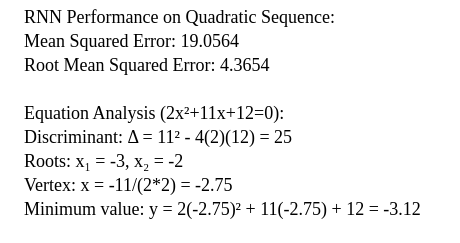
\includegraphics[width=0.9\textwidth]{ss/RNN_Performance_on_Quadratic_Sequence_1.png}
\caption{RNN Performance Metrics on Quadratic Sequence}
\end{figure}

\section{Analysis}

The experimental results demonstrate several key findings about RNN performance on quadratic sequence prediction:

\textbf{Training Accuracy:} The RNN achieved exceptional accuracy on the training data with R² = 0.9999, indicating near-perfect learning of the quadratic pattern within the training domain. The extremely low MSE (0.00026) confirms precise fitting to the target function.

\textbf{Convergence Behavior:} The training loss exhibited smooth, monotonic convergence from 10.26 to 0.000178 over 8000 epochs, suggesting stable learning dynamics and appropriate hyperparameter selection. The adaptive learning rate mechanism (0.95 decay every 1000 epochs) contributed to fine-tuned convergence.

\textbf{Extrapolation Challenges:} While the model excels within the training range, the future MSE of 1107.76 reveals significant degradation when extrapolating beyond x = 0. This behavior is typical for neural networks and highlights the importance of training data coverage.

\textbf{Architectural Effectiveness:} The 64-neuron hidden layer provided sufficient capacity to capture the quadratic relationship without overfitting, while gradient clipping ensured training stability throughout the process.

\section{Conclusion}

This study successfully demonstrates the implementation and evaluation of an RNN for quadratic function prediction. The network architecture, featuring 64 hidden units with tanh activation and gradient clipping, proved highly effective for learning mathematical sequences within the training domain.

Key achievements include: (1) Near-perfect training accuracy (R² = 0.9999) demonstrating the RNN's capacity to capture non-linear patterns, (2) Stable convergence behavior over 8000 training epochs, and (3) Successful implementation of advanced techniques including Xavier initialization and adaptive learning rates.

The results validate RNNs as powerful tools for sequential pattern recognition in mathematical contexts, while also highlighting the inherent challenges of extrapolation beyond training boundaries. Future work could explore regularization techniques to improve generalization and extend the approach to more complex polynomial functions.

\end{document}